\section{INTRODUCTION}\label{introduction}

% fill missing citations

Most reaching tasks in control and robotics can be phrased as \emph{tracking} problems, where the dynamical system needs to follow a certain predefined trajectory in order to reach the goal state. Robotic table tennis in particular~\cite{Muelling13} consists of planning, generating and executing a series of such (episodic) single stroke trajectories. These trajectories need to be followed very closely with motor commands in practice, in order to return the ball to the goal position. 

% maybe cite Jens' review paper
There have been many attempts in the reinforcement learning (RL)~\cite{Sutton98} and control literature to learn robotic tasks directly. Value function based methods take advantage of duality to solve the Bellman's equation but suffer from the initial bias or representation in estimating the value function and do not scale well to high dimensions. Policy search based RL methods (e.g.,~\cite{Kober08}, \cite{Peter10}, \cite{Theodorou10}, \cite{Deisenroth11}) directly solve the Bellman's equation in a parameterized policy space and can be more effective in practice~\cite{Kober13}. 

Dynamic Movement Primitives (DMP) are a kind of kinematic policy representation that leverages the dynamical systems approach to modify the spring dynamics with a forcing term that enables it to mimic an executed trajectory. They include an internal phase or clock that ensures the convergence of the movement primitive to a goal state~\cite{Ijspeert13}, \cite{Schaal07}. DMPs do not suffer from the curse of dimensionality as the number of parameters (weights) grow linearly with dimension. However, approximation and control errors in robotic platforms make the application of DMPs less useful in practice. Small changes to DMPs can often make them more useful.

Motor primitives can be modulated in different ways to adapt to unforeseen events or to ensure the optimal execution of required tasks. They work particularly well with episodic policy search methods that modify the weights of the forcing term based on the rewards received in every episode. By adapting the DMP that was initialized with imitation learning e.g., with kinesthetic teach-in~\cite{Muelling13}, RL approaches are able to achieve complex robotic tasks, such as ball-in-a-cup~\cite{Kober09}. However model-free methods (e.g., \cite{Kober08}, \cite{Peter10}) require many iterations to converge, whereas more data-efficient approaches such as~\cite{Deisenroth11} suffer from computational runtime difficulties and cannot be implemented in real-time robotics tasks. Optimality of the converged policy cannot be guaranteed by these methods.
% maybe mention reference trajectory?
% model-free ? PILCO claims to be 'model-based', yet it learns from scratch. It only 'learns' a model, but it is unbiased.

% inaccurate ?
Inspired by the successes (and failures) of these previous approaches, the research question that we tackle in this article consists of the following:
%
\begin{itemize}
\item How can we execute optimally hitting movement primitives either in table tennis or a similar reaching task e.g., putting in golf.
%
\item More specifically, when we have modelling inaccuracies, how should we modify a DMP $\dmp(t)$ such that the robot executes a desired hitting motion?
\end{itemize}
%
\begin{figure}[b!]
\center
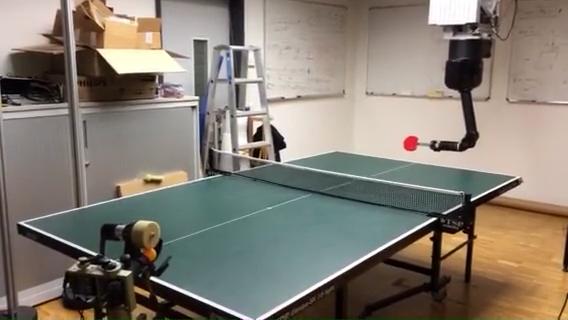
\includegraphics[scale=0.4]{robot1.png}			
\caption{Robotic table tennis setup with the ball-launcher throwing balls to the robot. In order to hit the ball to a desired position on the opponent's court, we give the robot reference trajectories that facilitate the right striking motion. We can teach the robot such trajectories via kinesthetic teach-in.}
\label{robot}
\end{figure}
%
% maybe include P. Abbeel's work on inaccurate models
\noindent We believe that learning in robotics tasks can be performed much more efficiently by taking advantage of existing imperfect models and reference trajectories. % optimality issues can be alleviated with given reference trajectories. 

Iterative Learning Control (ILC) is a fundamental approach in control theory developed to track (time-varying) reference trajectories. It has been used successfully to follow trajectories under unknown repeating disturbances and model mismatch \cite{Bristow06}. In ILC, control inputs are adjusted at each episode in a feedforward fashion. The goal is to drive the deviations from the trajectory to zero. 
% or equivalently references

In this article, we combine Iterative Learning Control with movement primitives by using ILC as a learning method to adapt the weights of the DMPs. This way we ensure a safe, reliant and robust way to track reference trajectories, with important applications in optimally hitting and striking motions. As opposed to model-free policy search approaches, we make full use of the known, albeit inexact, robot dynamics and inverse dynamics models, which helps us to quickly achieve the desired performance requirements. We validate the performance of the approach in two hitting tasks, and compare with existing episodic-RL approaches.
% nominal model instead of known, albeit inexact?

Our contributions can be summarized as follows: we form a link between the ILC literature and the movement primitives by systematically formulating an iterative update of the DMP weights. We form a coherent learning framework and present new motor primitive update laws. These are studied in detail and the implemented ILC algorithm~$\alg$ is shown to perform better than existing RL approaches in two hitting tasks, putting and table tennis.

In Section~\ref{relatedWork} we mention related work, especially the state of the art approaches in hitting and reaching tasks. In Section~\ref{problemStatement} we state the problem and introduce motor primitive update laws, relating them to the existing optimization-based ILC approaches. We formulate one of these update laws, called $\alg$, in algorithmic form in Section~\ref{algorithm}. In Section~\ref{experiments} we evaluate $\alg$ in two robotic reaching tasks: putting motion in golf and the striking motions in table tennis. We show that the method outperforms the state-of-the-art RL-based approaches \emph{REPS} and \emph{PI$^{2}$}. Finally in Section~\ref{conclusion} we discuss the strengths and weaknesses of our method and conclude with brief mentions of promising future research directions.

\subsection{Related Work}\label{relatedWork}

% mention the ILC paper of Peter Abbeel
Dynamic movement primitives belong to the class of movement primitives~\cite{Flash85}. Movement primitives are a kinematics-based approach to keep the learning tasks in high-dimensional tasks, such as in humonoid robotics, tractable. Like the options framework in Markov Decision Processes, they aim at reducing the curse of dimensionality in complex human-like robotics tasks. The first dynamical systems based formulation of movement primitives appeared in~\cite{Ijspeert02}. A good review with alternative and variant formulations is given in~\cite{Ijspeert13}.

% Policy search methods
One of the first examples of policy search based methods that modify the parameters of movement primitives is the \emph{POWER} algorithm~\cite{Kober08}. \emph{PI$^{2}$} algorithm has a very similar implementation in~\cite{Theodorou10} and episodic-\emph{REPS}~\cite{Peter10} is actually equivalent to \emph{POWER}.

Iterative Learning Control started out in the 1980s with the work of Arimoto et al.~\cite{Arimoto84} as one of the first to define the genre with the PD-type update law. See~\cite{Bristow06} and \cite{Moore99} for reviews. Monotonic convergence and stability guarantees are of central importance for the practical usefulness of ILC algorithms. They are shown for example in~\cite{Bristow06}, \cite{Norrloef02}, \cite{Longman2000}.

% ILC work - mention Angela's work
As an example of a more sophisticated method than the PD-type update laws, Schoellig et al.~\cite{Schoellig12} applied a Kalman-filter based convex optimization rule in the framework of ILC and showed its performance in quadrocopter flight. An EM-based update law was given in~\cite{Berg10} where an impressive application of ILC to a robotic surgical task was presented.
% This work however lacks any guarantees of monotonic convergence

% DMPs using Iterative Learning Control
DMPs have been also combined in a bimanual robotics task with ILC~\cite{Gams13} where force feedback is used to enable compliant interaction with objects in an unknown environment. ILC is here used to learn a coupling term between the two arm trajectories. To the best of our knowledge, ILC has not been used so far to modify the weights of the movement primitives.
% used to modulate the DMP and learn ...

\subsection{Problem Statement}\label{problemStatement}

The goal in trajectory tracking is to track a given reference $\traj(t), \ 0 \leq t \leq T \ $ by applying the control inputs $\sysInput(t)$. The reference trajectory in our case enables the \emph{optimal} execution of hitting and striking motions, e.g., forehand and backhand strikes in (table) tennis. We assume that such optimal trajectories are available to us, either through kinesthetic teach-in or computed recursively.
% talk about feasibility.
% reference needed? Dynamic programming?

% subsubsection entitled 'modelling assumptions'?
% talk of model-free regression update of DMP there maybe?

Consider the nonlinear robot dynamics of the form
%
\begin{equation}
\begin{aligned}
\ddot{\joint} &= \dynamics(\joint,\dot{\joint},\sysInput), \\
\ddot{\joint} &= \vec{M}^{-1}(\joint)\{ \vec{\tau}(\sysInput) - \vec{C}(\joint,\dot{\joint})\dot{\joint} - \vec{G}(\joint)\} + \dist(\joint,\dot{\joint}),\\
\end{aligned}
\label{dynamics}
\end{equation}
%
\noindent where on the right hand side are the terms due to the rigid body dynamics model and $\dist(\joint,\dot{\joint})$ are the (unmodeled) disturbances that act on the robot, such as viscous friction, stiction, etc. This system can be linearized around a given joint space trajectory $\traj(t), \ 0 \leq t \leq T$ with nominal inputs $\trjInput(t)$ calculated using the inverse dynamics model. We then obtain the following linear time varying (LTV) representation
%
\begin{equation}
\begin{aligned}
\dot{\error} = \vec{A}^{c}(t)\error(t) + \vec{B}^{c}(t)\linInput(t) + \linDist(t,\sysInput),
\end{aligned}
\label{LTV}
\end{equation}
%
\noindent where the state error is denoted as $\error(t) = \state(t) - \traj(t)$, the joint angles and velocities are $\state = [\joint,\dot{\joint}]^{\mathrm{T}}$, $\linInput(t) = \sysInput(t) - \trjInput(t)$ and the continuous time varying matrices are
%
\begin{equation}
\begin{aligned}
\vec{A}^{c}(t) &= \at{\frac{\partial{\dynamics}}{\partial{\state}}}{(\traj(t),\trjInput(t))}, \\
\vec{B}^{c}(t) &= \at{\frac{\partial{\dynamics}}{\partial{\sysInput}}}{(\traj(t),\trjInput(t))}.
\end{aligned}
\label{LTVmatrices}
\end{equation}
%
% what about estimation errors, i.e. sensor errors ...
\noindent In the error dynamics \eqref{LTV} the additional term $\linDist(t,\sysInput)$ accounts for the disturbances and the effects of the linearization. We can discretize (\ref{LTV}-\ref{LTVmatrices}) with step size $\delta$, $N = T/\delta$ and step index $j = 1, \ldots, N$ to get the following discrete linear system
%
\begin{equation}
\begin{aligned}
\error_{j+1} = \vec{A}_j\error_j + \vec{B}_j\linInput_j + \linDist_j(\sysInput_1, \ldots, \sysInput_j),
\end{aligned}
\label{discreteLTV}
\end{equation}
%
\noindent where the matrices $\vec{A}, \vec{B}$ are the discretizations of \eqref{LTVmatrices}. Conventional ILC algorithms learn to compensate for the errors by iterating the control inputs $\sysInput$ with an update law.